% --------------------------------------------------------------
% This is all preamble stuff that you don't have to worry about.
% Head down to where it says "Start here"
% --------------------------------------------------------------
 
\documentclass[12pt]{article}
 
\usepackage[margin=1in]{geometry} 
\usepackage{amsmath,amsthm,amssymb}
\usepackage{braket}
\usepackage{graphicx}
\usepackage{calligra}
\usepackage{calrsfs}
\usepackage{subcaption}
\usepackage{listings}
\newcommand{\N}{\mathbb{N}}
\newcommand{\Z}{\mathbb{Z}}
 
\newenvironment{theorem}[2][Theorem]{\begin{trivlist}
\item[\hskip \labelsep {\bfseries #1}\hskip \labelsep {\bfseries #2.}]}{\end{trivlist}}
\newenvironment{lemma}[2][Lemma]{\begin{trivlist}
\item[\hskip \labelsep {\bfseries #1}\hskip \labelsep {\bfseries #2.}]}{\end{trivlist}}
\newenvironment{exercise}[2][Exercise]{\begin{trivlist}
\item[\hskip \labelsep {\bfseries #1}\hskip \labelsep {\bfseries #2.}]}{\end{trivlist}}
\newenvironment{reflection}[2][Reflection]{\begin{trivlist}
\item[\hskip \labelsep {\bfseries #1}\hskip \labelsep {\bfseries #2.}]}{\end{trivlist}}
\newenvironment{proposition}[2][Proposition]{\begin{trivlist}
\item[\hskip \labelsep {\bfseries #1}\hskip \labelsep {\bfseries #2.}]}{\end{trivlist}}
\newenvironment{corollary}[2][Corollary]{\begin{trivlist}
\item[\hskip \labelsep {\bfseries #1}\hskip \labelsep {\bfseries #2.}]}{\end{trivlist}}
 
\begin{document}
 
% --------------------------------------------------------------
%                         Start here
% --------------------------------------------------------------
 
%\renewcommand{\qedsymbol}{\filledbox}
 
\title{HW8}
\author{Carl Mueller\\ %replace with your name
CSCI 5254 - Convex Optimization} %if necessary, replace with your course title
\maketitle

\subsection*{8.16}
\subsubsection*{a)}
\textbf{Gradient Method}

\begin{figure}[ht]
    \centering
    \begin{subfigure}{0.4\textwidth} % width of left subfigure
        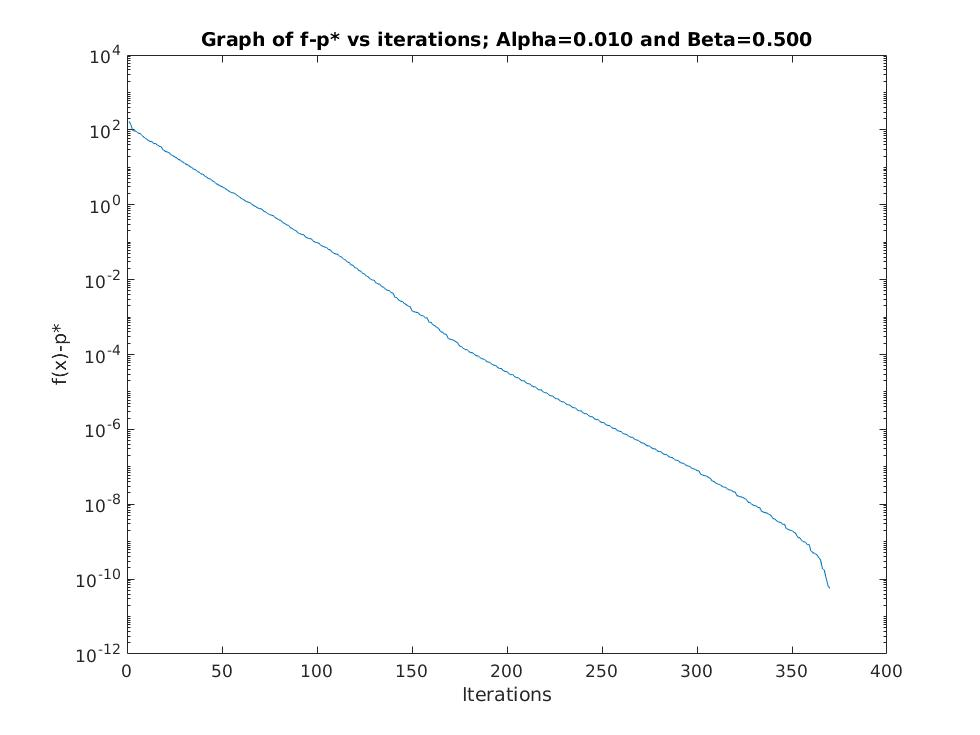
\includegraphics[width=\textwidth]{f_alpha_01_beta_50.jpg}
    \end{subfigure}
    \vspace{1em} % here you can insert horizontal or vertical space
    \begin{subfigure}{0.4\textwidth} % width of right subfigure
        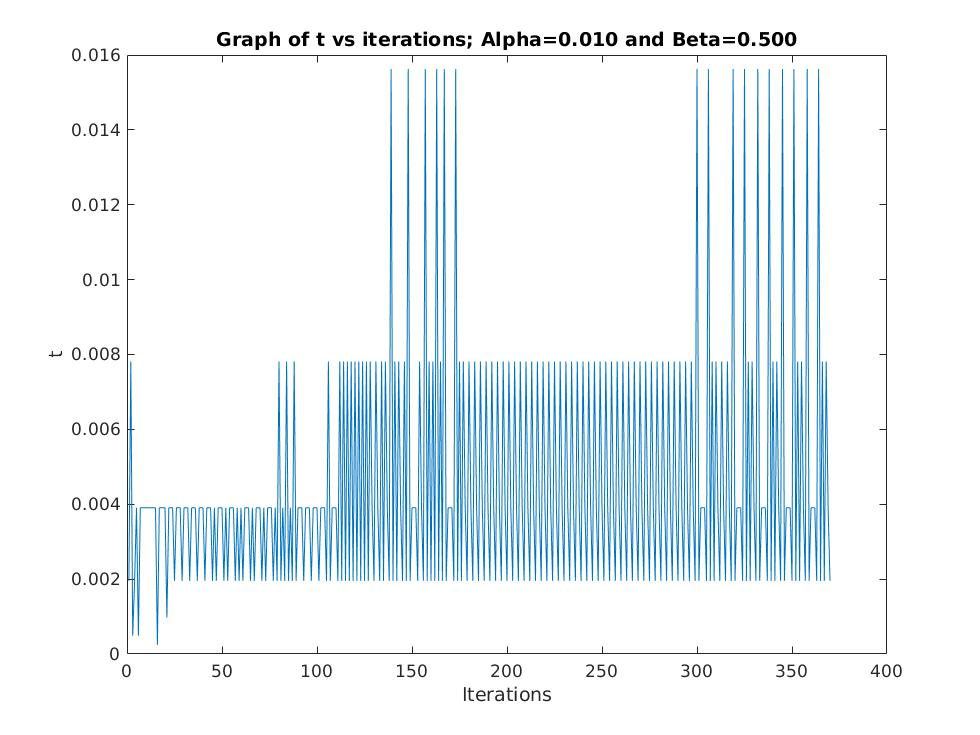
\includegraphics[width=\textwidth]{t_alpha_01_beta_50.jpg}
    \end{subfigure}
    \caption{ALPHA=.01, BETA=.5} % caption for whole figure
\end{figure}
\begin{figure}[ht]
    \centering
    \begin{subfigure}{0.4\textwidth} % width of left subfigure
        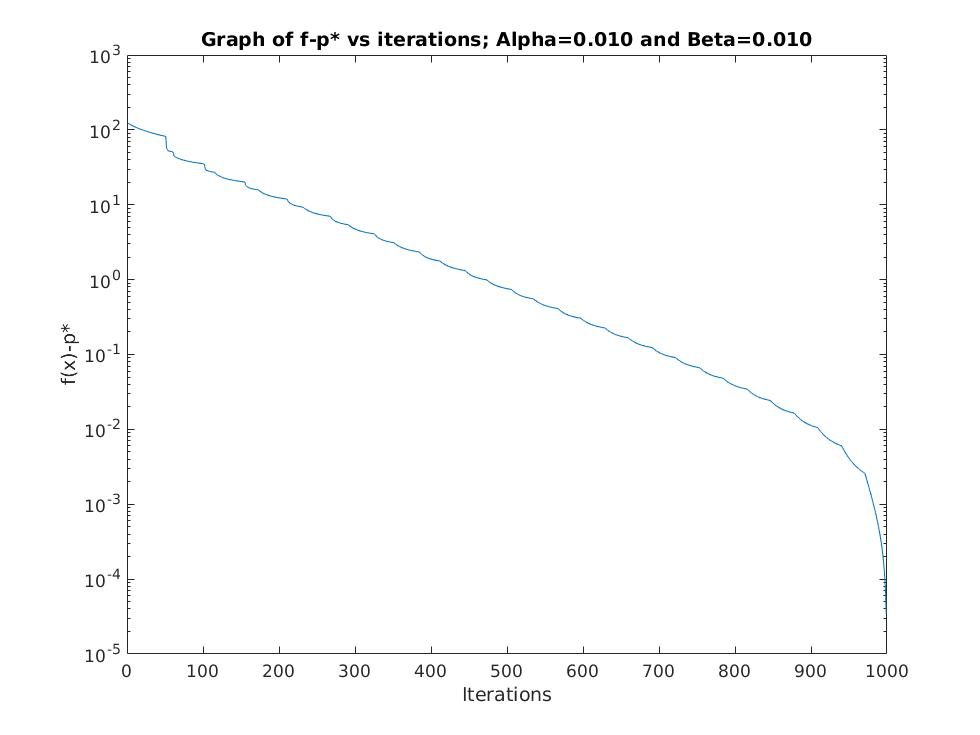
\includegraphics[width=\textwidth]{f_alpha_01_beta_01.jpg}
    \end{subfigure}
    \vspace{1em} % here you can insert horizontal or vertical space
    \begin{subfigure}{0.4\textwidth} % width of right subfigure
        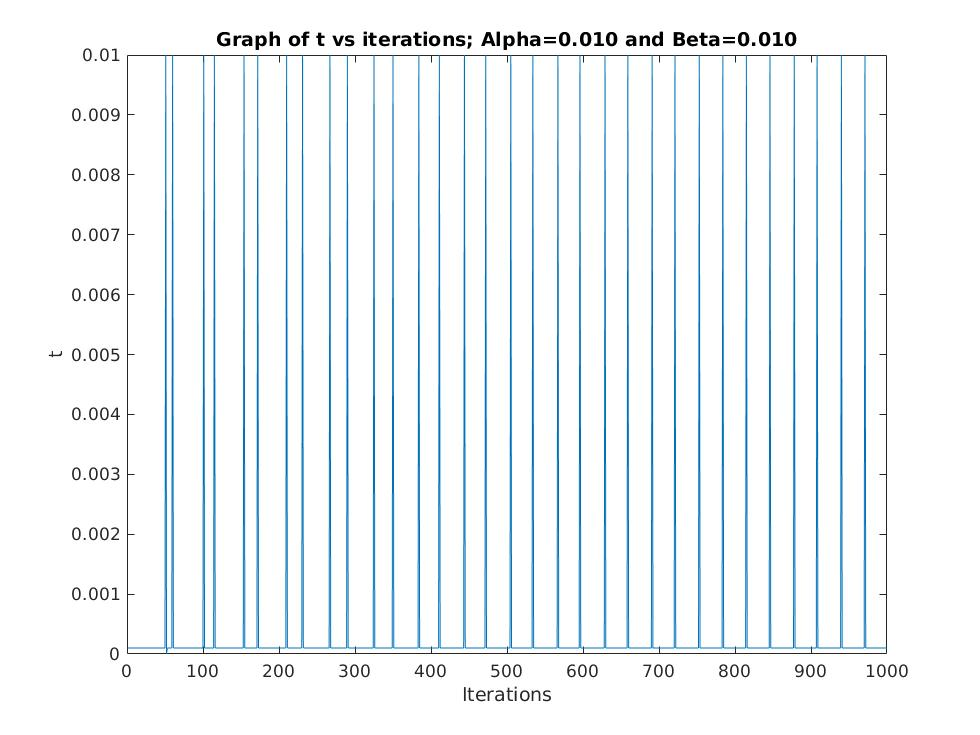
\includegraphics[width=\textwidth]{t_alpha_01_beta_01.jpg}
    \end{subfigure}
    \caption{ALPHA=.01, BETA=.01} % caption for whole figure
\end{figure}
\begin{figure}[ht]
    \centering
    \begin{subfigure}{0.4\textwidth} % width of left subfigure
        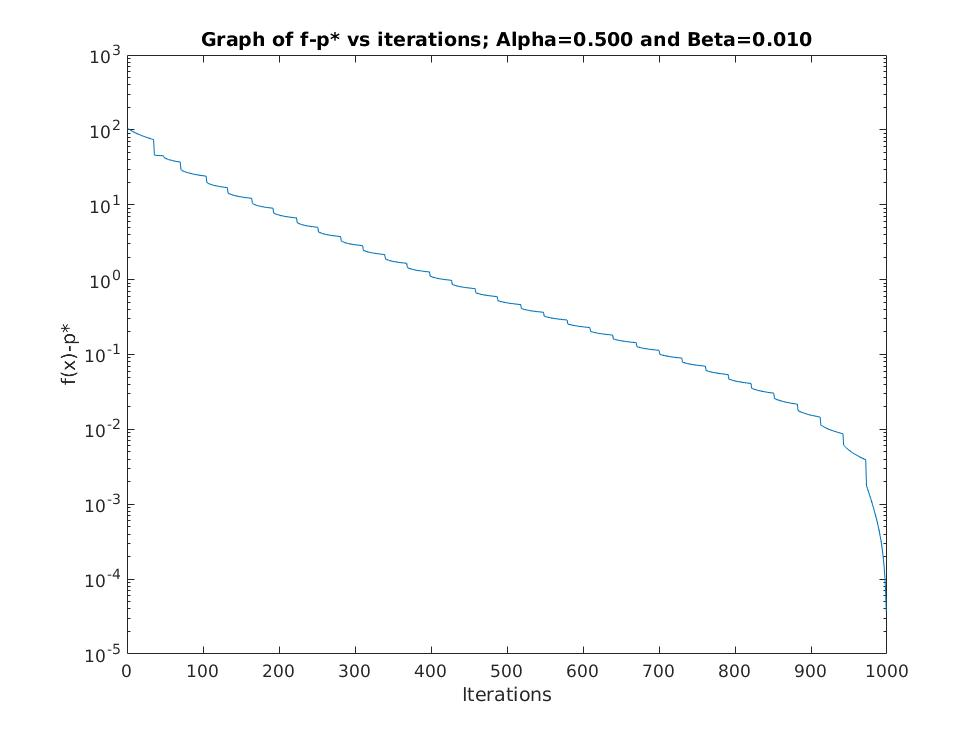
\includegraphics[width=\textwidth]{f_alpha_50_beta_01.jpg}
    \end{subfigure}
    \vspace{1em} % here you can insert horizontal or vertical space
    \begin{subfigure}{0.4\textwidth} % width of right subfigure
        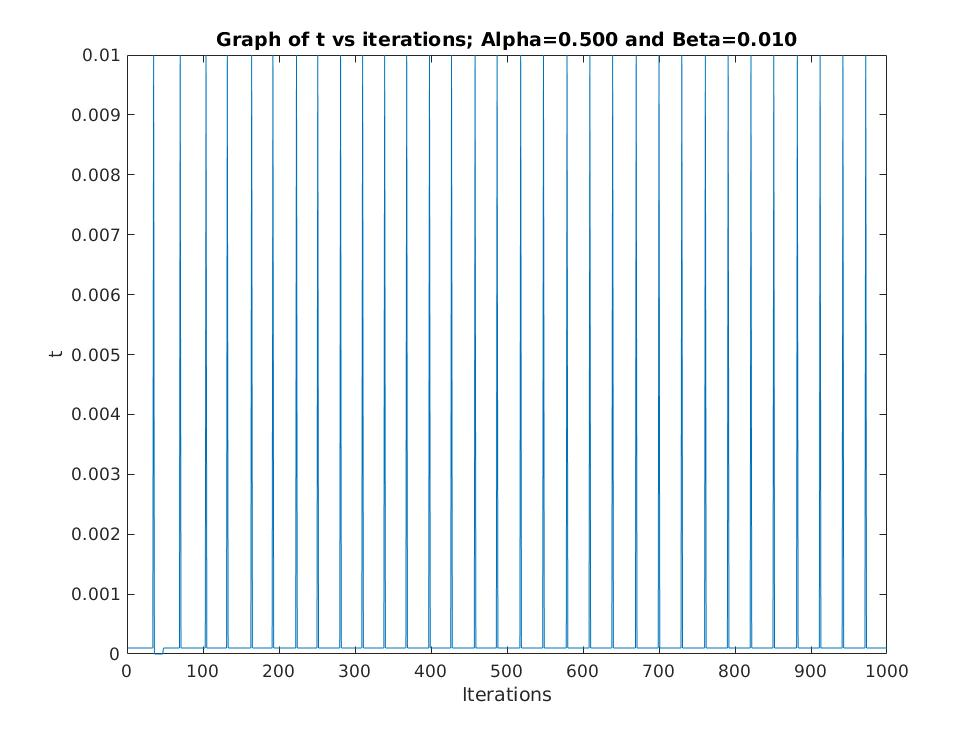
\includegraphics[width=\textwidth]{t_alpha_50_beta_01.jpg}
    \end{subfigure}
    \caption{ALPHA=.50, BETA=.01} % caption for whole figure
\end{figure}
\begin{figure}[ht]
    \centering
    \begin{subfigure}{0.4\textwidth} % width of left subfigure
        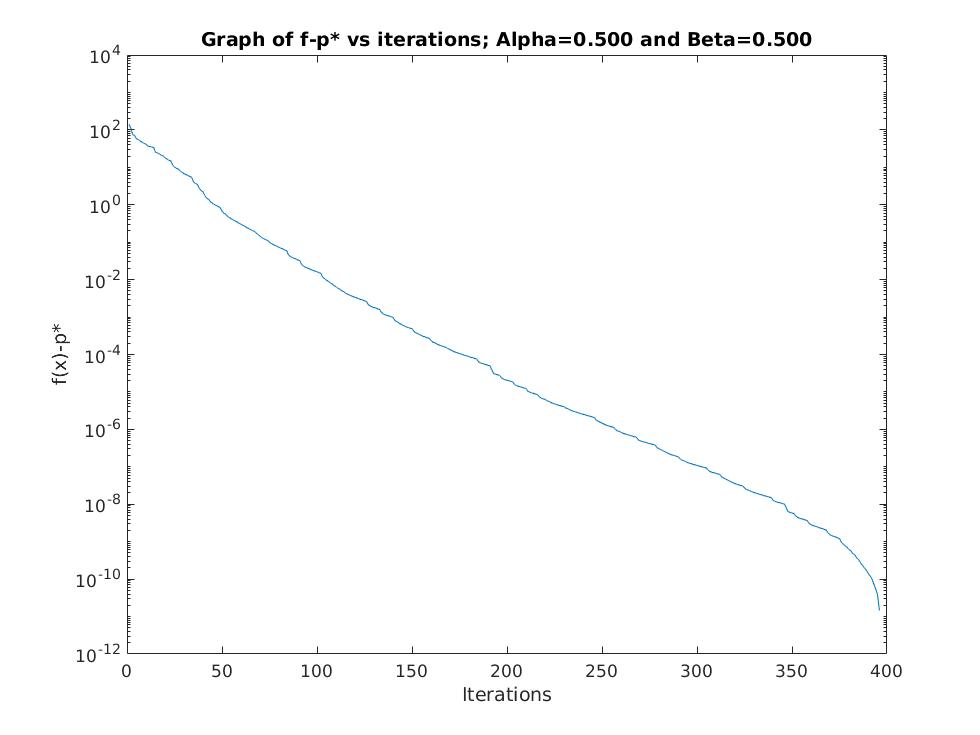
\includegraphics[width=\textwidth]{f_alpha_50_beta_50.jpg}
    \end{subfigure}
    \vspace{1em} % here you can insert horizontal or vertical space
    \begin{subfigure}{0.4\textwidth} % width of right subfigure
        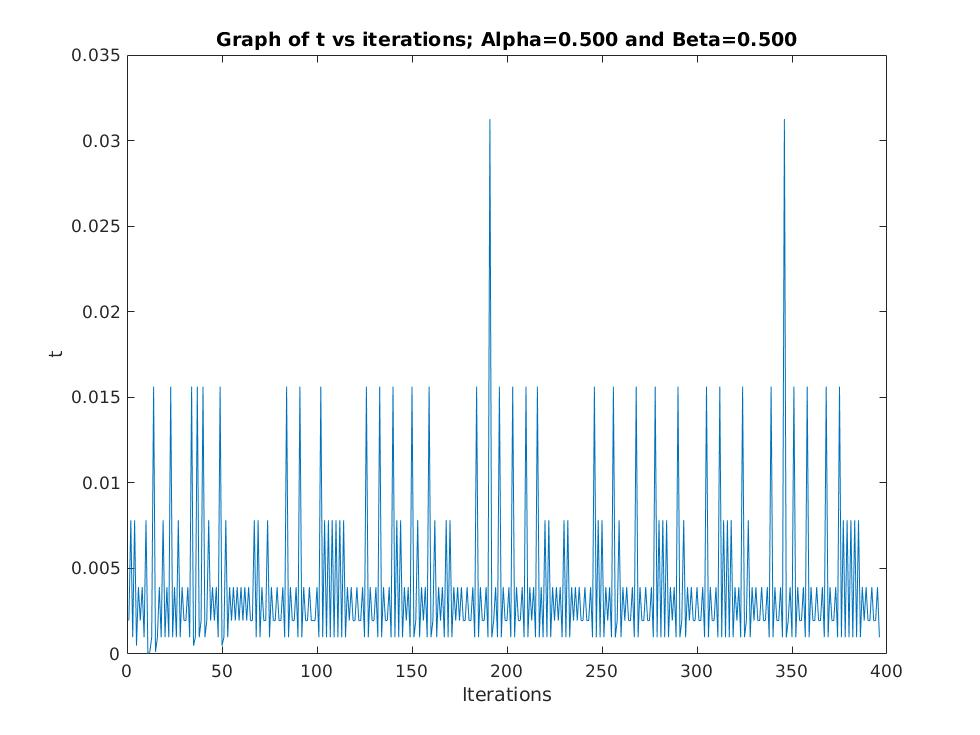
\includegraphics[width=\textwidth]{t_alpha_50_beta_50.jpg}
    \end{subfigure}
    \caption{ALPHA=.50, BETA=.50} % caption for whole figure
\end{figure}

\begin{lstlisting}
iter = 1000;
nu = .0001;
beta = .01;
alpha = .5;
n = 100;
m = 200;
x = zeros(n, 1);
A = randn(m,n);

V = []
I = []
T = []
for i = 1:iter
    % function evaluation
    f = -sum(log(1-A*x))-sum(log(1+x)) - sum(log(1-x));
    % gradient
    grad = A'*(1./(1-A*x)) - 1./(1+x) + 1./(1-x);
    % breaking criterion using nu as threshold
    if norm(grad) < nu
        break
    end
    % Gradient direction.
    dir = -grad;
    % second compoenent of backtracking
    fprime = grad'*dir;
    t = 1; 
    while ((max(A*(x+t*dir)) >= 1) || (max(abs(x+t*dir)) >= 1))
        t = beta*t;
    end
    % backtracking algorithm
    while ( -sum(log(1-A*(x+t*dir))) - sum(log(1-(x+t*dir).^2)) > f + alpha*t*fprime )
        t = beta*t;
    end
    % update step
    x = x+t*dir;
    T = [T; t]
    V = [V; f];
    I = [I ; i]
end

f_minus_p = [];
for i = 1:length(V)
    diff = V(i) - f
    f_minus_p = [f_minus_p; diff]
end
f_minus_p
f
figure(1)
plot(I,f_minus_p);
set(gca,'yscale','log');
titlestr = "Graph of f-p* vs iterations; Alpha=%0.3f and Beta=%0.3f";
str = sprintf(titlestr,alpha,beta);
title(str);
xlabel("Iterations");
ylabel("f(x)-p*");

figure(2)
plot(I,T);
titlestr = "Graph of t vs iterations; Alpha=%0.3f and Beta=%0.3f";
str = sprintf(titlestr,alpha,beta);
title(str);
xlabel("Iterations");
ylabel("t");
\end{lstlisting}

\subsubsection*{b)}
\textbf{Newton's Method}\\
This approach clearly takes many less iterations and is always terminated based on the quit criteria rather than the max number of iterations. 

\begin{figure}[ht]
    \centering
    \begin{subfigure}{0.4\textwidth} % width of left subfigure
        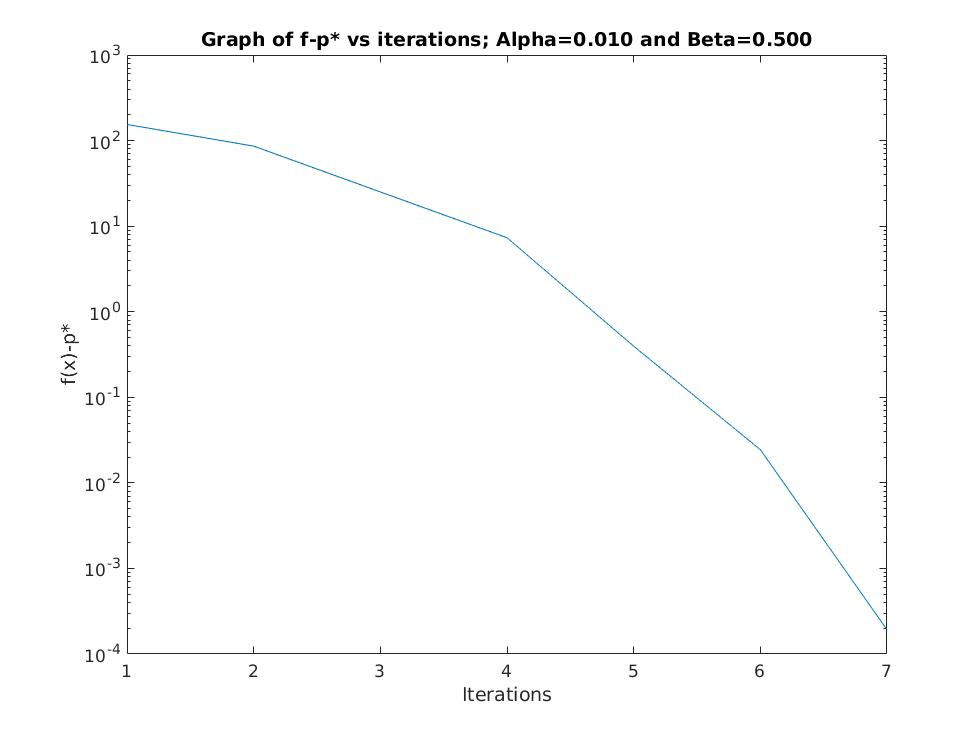
\includegraphics[width=\textwidth]{newton_f_alpha_01_beta_50.jpg}
    \end{subfigure}
    \vspace{1em} % here you can insert horizontal or vertical space
    \begin{subfigure}{0.4\textwidth} % width of right subfigure
        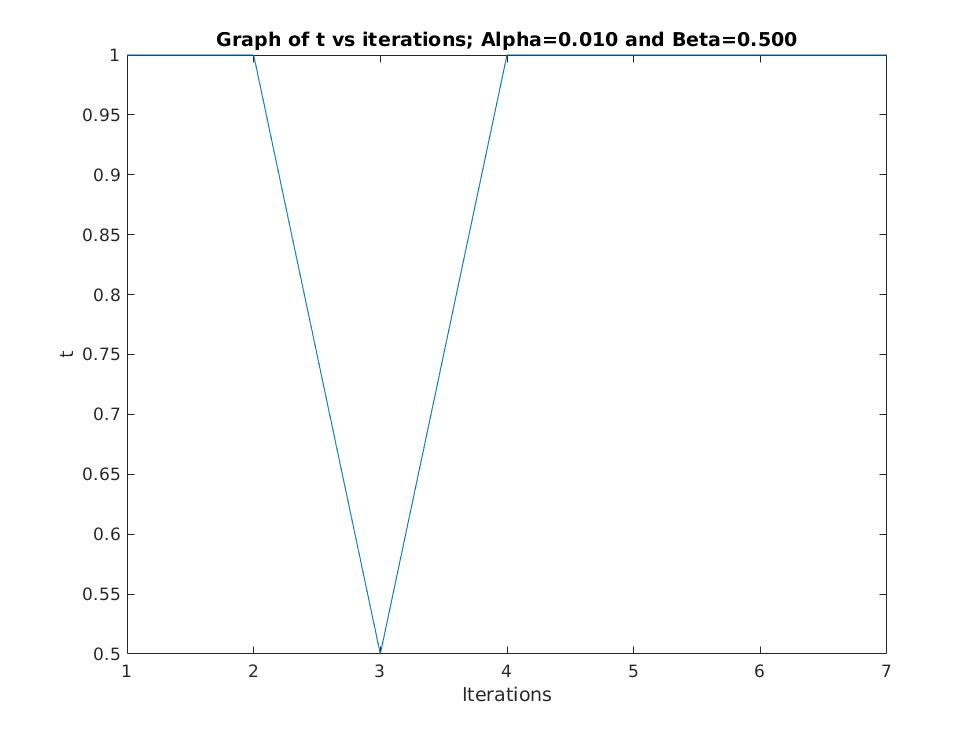
\includegraphics[width=\textwidth]{newton_t_alpha_01_beta_50.jpg}
    \end{subfigure}
    \caption{ALPHA=.01, BETA=.5} % caption for whole figure
\end{figure}
\begin{figure}[ht]
    \centering
    \begin{subfigure}{0.4\textwidth} % width of left subfigure
        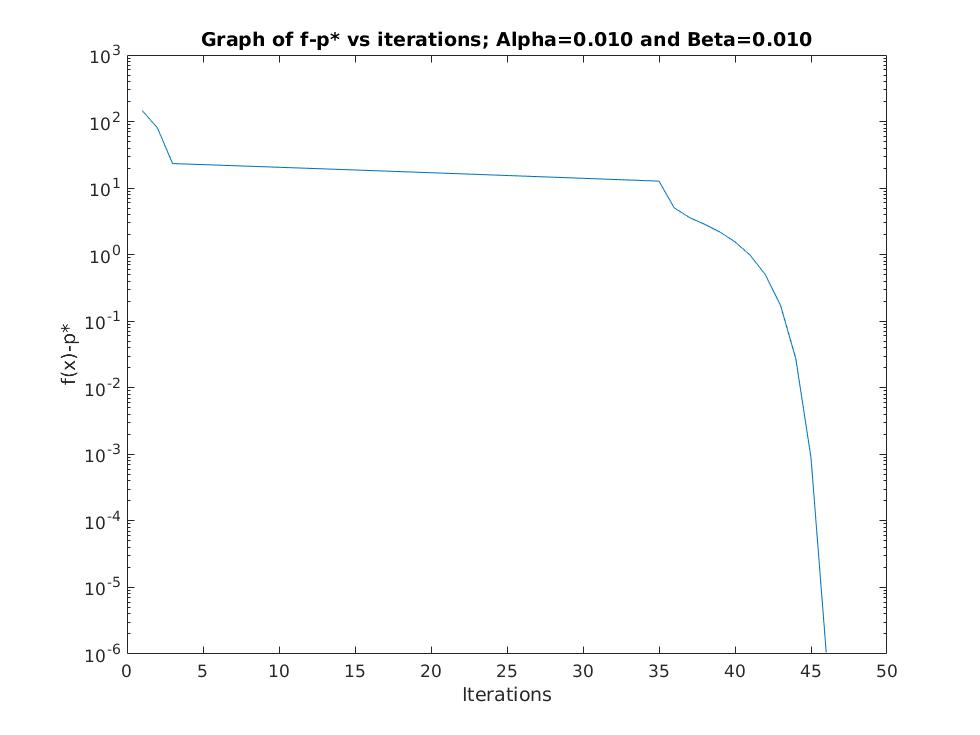
\includegraphics[width=\textwidth]{newton_f_alpha_01_beta_01.jpg}
    \end{subfigure}
    \vspace{1em} % here you can insert horizontal or vertical space
    \begin{subfigure}{0.4\textwidth} % width of right subfigure
        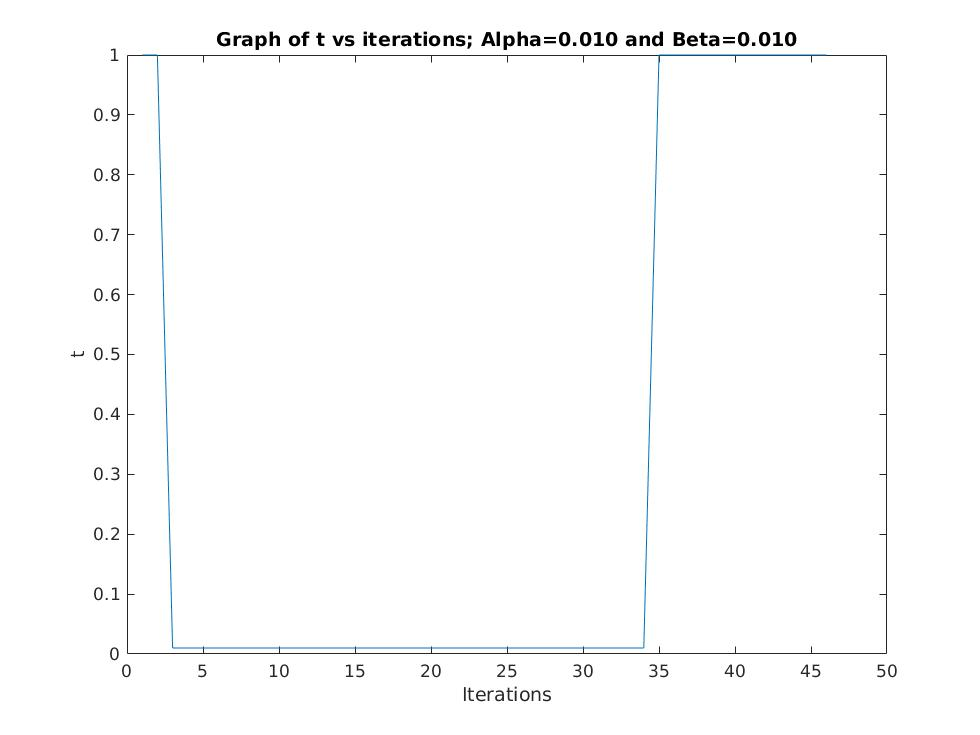
\includegraphics[width=\textwidth]{newton_t_alpha_01_beta_01.jpg}
    \end{subfigure}
    \caption{ALPHA=.01, BETA=.01} % caption for whole figure
\end{figure}
\begin{figure}[ht]
    \centering
    \begin{subfigure}{0.4\textwidth} % width of left subfigure
        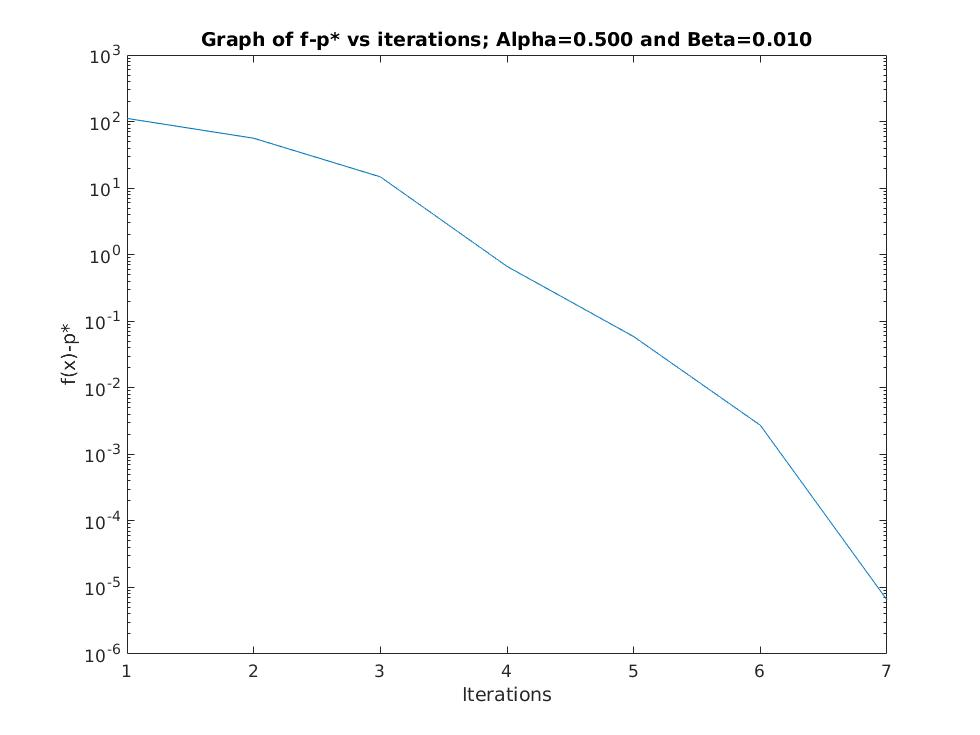
\includegraphics[width=\textwidth]{newton_f_alpha_50_beta_01.jpg}
    \end{subfigure}
    \vspace{1em} % here you can insert horizontal or vertical space
    \begin{subfigure}{0.4\textwidth} % width of right subfigure
        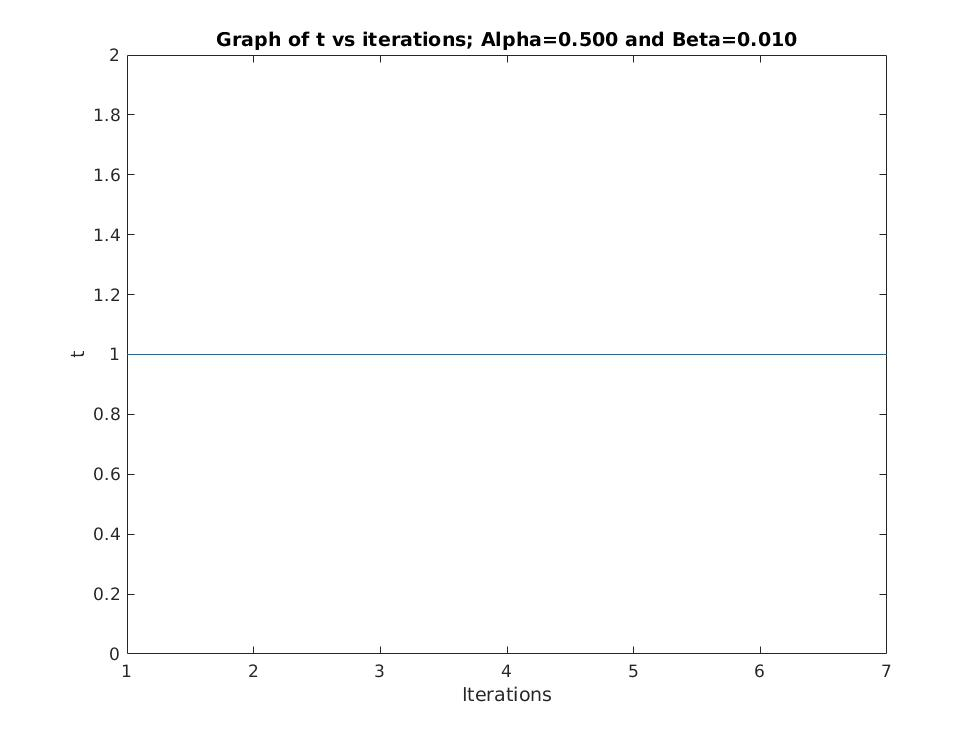
\includegraphics[width=\textwidth]{newton_t_alpha_50_beta_01.jpg}
    \end{subfigure}
    \caption{ALPHA=.50, BETA=.01} % caption for whole figure
\end{figure}
\begin{figure}[ht]
    \centering
    \begin{subfigure}{0.4\textwidth} % width of left subfigure
        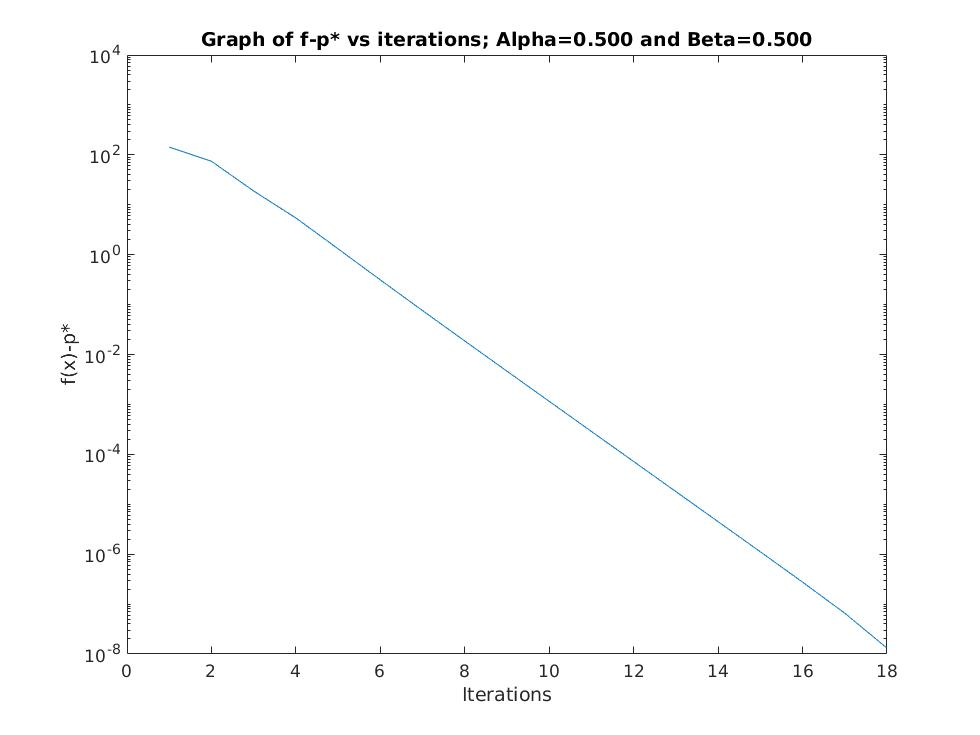
\includegraphics[width=\textwidth]{newton_f_alpha_50_beta_50.jpg}
    \end{subfigure}
    \vspace{1em} % here you can insert horizontal or vertical space
    \begin{subfigure}{0.4\textwidth} % width of right subfigure
        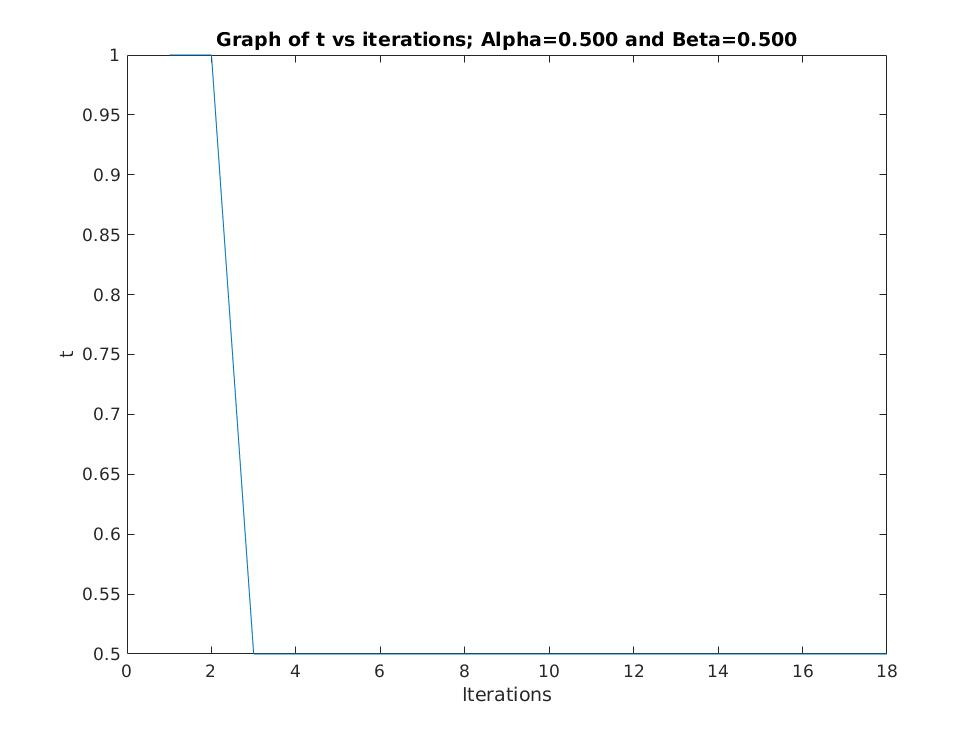
\includegraphics[width=\textwidth]{newton_t_alpha_50_beta_50.jpg}
    \end{subfigure}
    \caption{ALPHA=.50, BETA=.50} % caption for whole figure
\end{figure}

\begin{lstlisting}
iter = 1000;
nu = .00000001;
beta = .01;
alpha = .50;
n = 100;
m = 200;
x = zeros(n, 1);
A = randn(m,n);


x = zeros(n,1);

V = []
I = []
T = []
for i = 1:iter
    f = -sum(log(1-A*x)) - sum(log(1+x)) - sum(log(1-x));
    d = 1./(1-A*x);
    % first order derivative
    grad = A'*d - 1./(1+x) + 1./(1-x);
    % second order derivative i.e. hessian
    hessian = A'*diag(d.^2)*A + diag(1./(1+x).^2 + 1./(1-x).^2);
    % direction
    dir = -hessian\grad;
    % lambda^2 i.e decrement
    lambda_2 = grad'*dir;
    t = 1; 
    while ((max(A*(x+t*dir)) >= 1) || (max(abs(x+t*dir)) >= 1))
        t = beta*t;
    end
    % breaking criteria
    if abs(lambda_2) < nu
        break;
    end
    % backtracking algorithm
    while ( -sum(log(1-A*(x+t*dir))) - sum(log(1-(x+t*dir).^2)) > f + alpha*t*lambda_2 )
        t = beta*t;
    end
    % update step
    x = x+t*dir;
    V = [V; f];
    I = [I ; i];
    T = [T; t];
end

f_minus_p = [];
for i = 1:length(V)
    diff = V(i) - f
    f_minus_p = [f_minus_p; diff]
end
f_minus_p
f
figure(1)
semilogy(I, f_minus_p)
titlestr = "Graph of f-p* vs iterations; Alpha=%0.3f and Beta=%0.3f";
str = sprintf(titlestr,alpha,beta);
title(str);
xlabel("Iterations");
ylabel("f(x)-p*");

figure(2)
plot(I,T);
titlestr = "Graph of t vs iterations; Alpha=%0.3f and Beta=%0.3f";
str = sprintf(titlestr,alpha,beta);
title(str);
xlabel("Iterations");
ylabel("t");
\end{lstlisting}

\subsection*{9.31}
\textbf{Delayed Hessian Update:}\\

\textbf{Code:}
\begin{lstlisting}
clear all;

iter = 1000;
nu = .00000001;
beta = .5;
alpha = .01;
n = 100;
m = 200;
x = zeros(n, 1);
A = randn(m,n);

GD = []

step = [1,5,10,20]
for N = 1:length(step)
    V = [];
    I = [];
    T = [];
    for i = 1:iter
        f = -sum(log(1-A*x)) - sum(log(1+x)) - sum(log(1-x));
        d = 1./(1-A*x);
        % first order derivative
        grad = A'*d - 1./(1+x) + 1./(1-x);
        % second order derivative i.e. hessian
        if i == 1 || mod(i, N) == 0
            hessian = A'*diag(d.^2)*A + diag(1./(1+x).^2 + 1./(1-x).^2);
        end
        % direction
        dir = -hessian\grad;
        % lambda^2 i.e decrement
        lambda_2 = grad'*dir;
        t = 1; 
        while ((max(A*(x+t*dir)) >= 1) || (max(abs(x+t*dir)) >= 1))
            t = beta*t;
        end
        % breaking criteria
        if abs(lambda_2) < nu
            break;
        end
        % backtracking algorithm
        while ( -sum(log(1-A*(x+t*dir))) - sum(log(1-(x+t*dir).^2)) > f + alpha*t*lambda_2 )
            t = beta*t;
        end
        % update step
        x = x+t*dir;
        V = [V; f];
        I = [I ; i];
        T = [T; t];
    end
    f_minus_p = [];
    for i = 1:length(V)
        diff = V(i) - f
        f_minus_p = [f_minus_p; diff]
    end
    GD = [GD ; {f, f_minus_p, V, I, T}]
    x = zeros(n, 1);
end


figure(1)
D = GD(1, :)
semilogy(D{4}, D{2})
hold on
D = GD(2, :)
semilogy(D{4}, D{2})
hold on
D = GD(3, :)
semilogy(D{4}, D{2})
hold on
D = GD(4, :)
semilogy(D{4}, D{2})
hold off
titlestr = "Graph of delayed Hessian Update for Netwon's method";
str = sprintf(titlestr,alpha,beta);
title(str);
xlabel("Iterations");
ylabel("f(x)-p*");
legend("Newton","N=5","N=10","N=20")
\end{lstlisting}
\begin{figure}[ht]
    \centering
    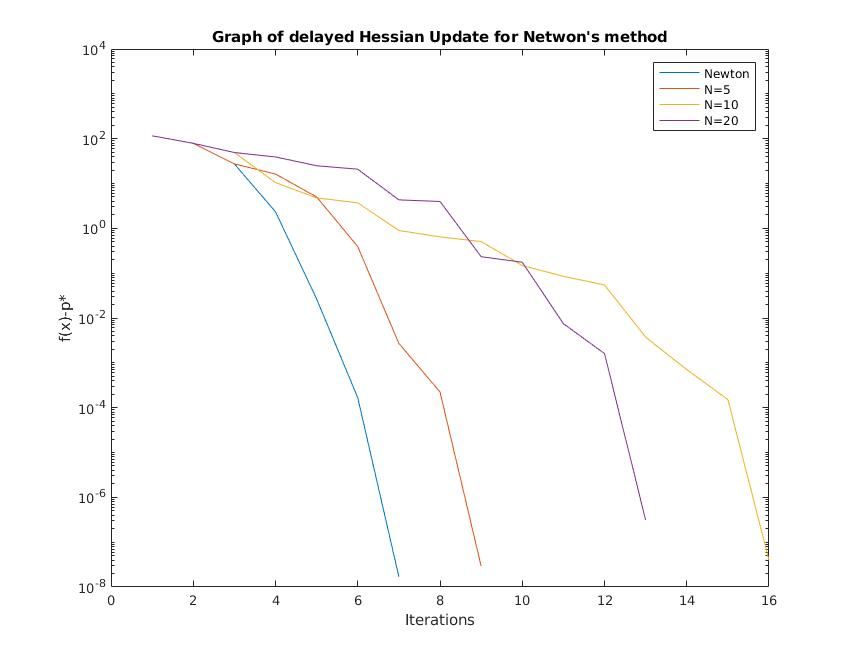
\includegraphics[width=\textwidth]{N_newton.jpg}
    \caption{Different iterations counts N until Hessian update.}
\end{figure}

\subsubsection{b)}
\subsection*{9.31}
\textbf{Delayed Hessian Update:}\\

\textbf{Code:}
\begin{lstlisting}

...

for i = 1:iter
    f = -sum(log(1-A*x)) - sum(log(1+x)) - sum(log(1-x));
    d = 1./(1-A*x);
    % first order derivative
    grad = A'*d - 1./(1+x) + 1./(1-x);
    % diagnal of the second order derivative i.e. hessian
   hessian = diag(diag(A'*diag(d.^2)*A + diag(1./(1+x).^2 + 1./(1-x).^2)));
    
...
\end{lstlisting}
\begin{figure}[ht]
    \centering
    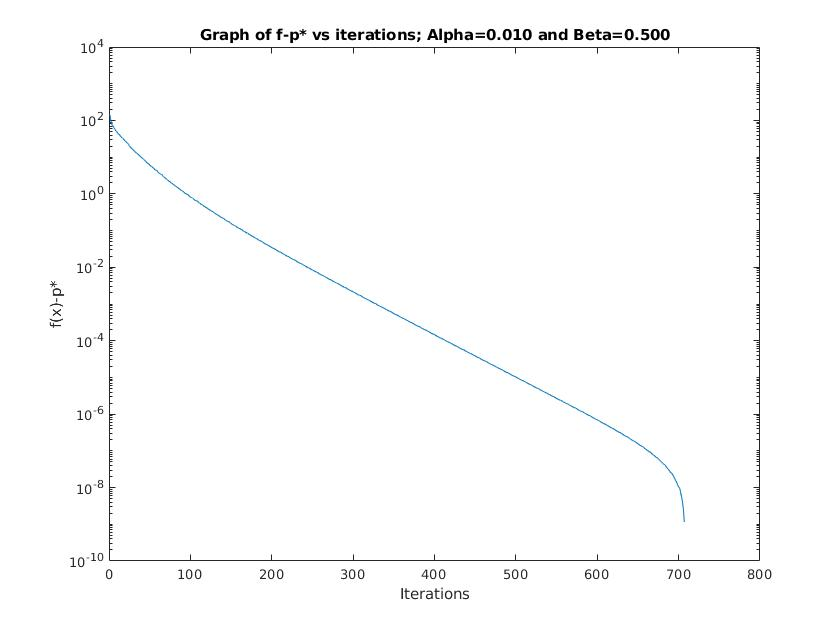
\includegraphics[width=\textwidth]{diagonal_hessian.jpg}
    \caption{Using the diagonal of the hessian. There is a clear increase in the required number of iterations}
\end{figure}
\break
\subsection*{11.1}
We are given the minimization problem:
\begin{equation*}
\begin{aligned}
& \underset{}{\text{minimize}}
& &x^2 + 1\\
& \text{subject to}\
& & 2 \le x \le 4
\end{aligned}
\end{equation*}
We used the log barrier approximation as follows:
$$\hat{I}(x) = -log(x-2) - log(4-x)$$
\textbf{Code:}
\begin{lstlisting}
t = [.01, .02, .04, .08, .16, .32, .64, 1.28, 2.56, 5.12, 10.80]

figure(1)
fplot(@(x) power(2,x)+1, [0,6])
hold on
for i = 1:length(t)
    fplot(@(x) power(2,x)+1 + (1/t(i))*(-log(x-2)-log(4-x)))
end
hold off
xlabel("x")
ylabel("function value")
title("Log Barrier of f for various t values.")
legend("t=.01","t=.02","t=.04","t=.08","t=.16","t=.32","t=.74","t=1.28","t=5.
\end{lstlisting}
\begin{figure}[ht]
    \centering
    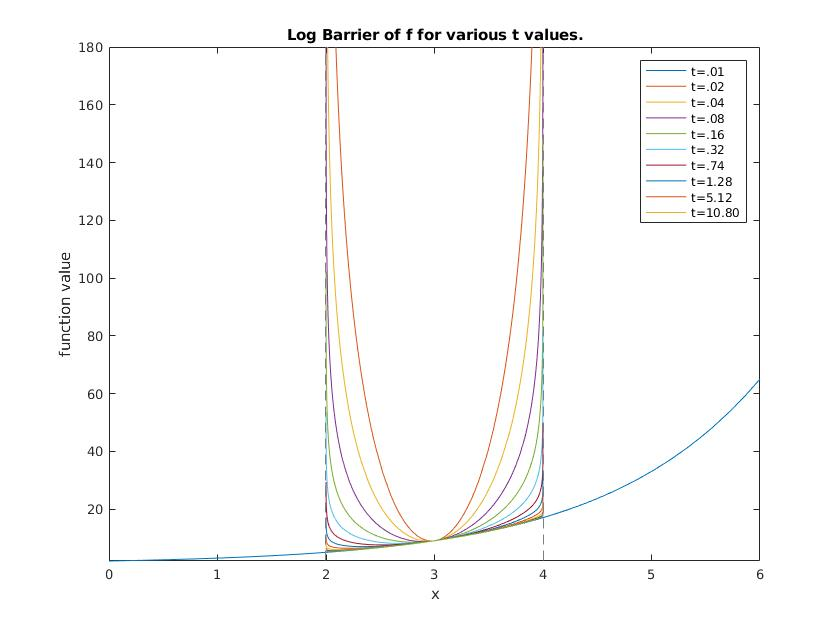
\includegraphics[width=\textwidth]{log_barrier.jpg}
    \caption{Log Barrier plotting verus f(x) for various t values.}
\end{figure}
\break
\subsection*{11.22}
We use the following optimization problem. We use  the bounds of our $x$ values of the constraints using $u$ and $l$ to constrain the log barrier of the rectangle.\\
Note: $A^+ = max(A, 0)$ and $A^- = max(-A, 0)$
\begin{equation*}
\begin{aligned}
& \underset{}{\text{minimize}}
& & -\sum_{i=1}^{n}log(u_i-l_i)\\
& \text{subject to}\
& & A^+u - A^-l \preceq b\\ 
&&& l \preceq u
\end{aligned}
\end{equation*}
\begin{equation*}
\begin{aligned}
& \psi = t-\sum_{i=1}^{n}log(u_i-l_i) - \sum_{i=1}^{n}log(b - A^+u_i + A^-l_i)\\
& \nabla \psi = t\begin{bmatrix} I\\ -I\end{bmatrix}diag(u-l)^{-1}\textbf{1} + \begin{bmatrix} -A^-^T \\ A^+^T\end{bmatrix}diag(b-A^+u+A^-l)^{-1}\textbf{1}\\
& \nabla^2 \psi = t\begin{bmatrix} I\\ -I\end{bmatrix}diag(u-l)^{-2}\begin{bmatrix} I\\ -I\end{bmatrix}^T + \begin{bmatrix} -A^-^T \\ A^+^T\end{bmatrix}diag(b-A^+u+A^-l)^{-2} \begin{bmatrix} -A^-^T\\ A^+^T\end{bmatrix}^T\\
\end{aligned}
\end{equation*}
% --------------------------------------------------------------
%     You don't have to mess with anything below this line.
% --------------------------------------------------------------
 
\end{document}